\documentclass[a4paper,12pt]{elsarticle}
\usepackage[a4paper]{geometry}
\usepackage[cm]{fullpage}
\usepackage{amsthm,amsmath,amssymb}
\usepackage{graphicx}
\usepackage{url}
\usepackage{natbib}
\bibliographystyle{abbrvnat}
\setcitestyle{authoryear,open={(},close={)}}
\usepackage{hyperref}

\numberwithin{equation}{section}
\theoremstyle{plain}
\newtheorem{theorem}{Theorem}[section]
\newtheorem{lemma}[theorem]{Lemma}
\newtheorem{proposition}[theorem]{Proposition}
\newtheorem{cor}[theorem]{Corollary}
\theoremstyle{definition}
\newtheorem{defi}[theorem]{Definition}
\newtheorem{example}[theorem]{Example}
\theoremstyle{remark}
\newtheorem{remark}[theorem]{Remark}
\numberwithin{equation}{section}

\newcommand{\Rd}{\mathbb R^d}
\newcommand{\spc}{\mathbb R}
\newcommand{\tim}{[0,\infty)}
\newcommand{\spctim}{\spc \times [0,\infty)}
\newcommand{\R}{\mathbb R}
\newcommand{\1}{\mathbf 1}
\newcommand{\pr}{\mathbf P}
\newcommand{\ex}{\mathbf E}
\newcommand{\del}{\partial}


\begin{document}

\begin{frontmatter}

\title{A Universal Algorithm for Continuum Limit Distributions of
Continuous Time Random Walks}
\author[UNSW]{Gurtek Gill}
\ead{rickygill01@gmail.com}
\author[UNSW]{Peter Straka}
\ead{p.straka@unsw.edu.au}
\address[UNSW]{School of Mathematics \& Statistics, UNSW Sydney}

\begin{abstract}
We propose a universal ``Semi-Markov algorithm'' for the computation of
probability distributions of Continuous Time Random Walks (CTRWs) and their
continuum limits.
The algorithm is universal in the following sense: Any CTRW continuum limit
can be mapped to a bivariate Langevin equation which tracks the cumulative sum
of jumps and waiting times, and given the coefficients of this Langevin
equation, the algorithm will compute the desired probability densities.
Besides subdiffusion with space- and time-dependent drift, this approach
covers subdiffusion with spatially varying exponent $\beta(x) \in (0,1)$ and
tempering parameter $\theta(x) \ge 0$, and subdiffusion with mixed (distributed)
order where the mixture can vary in space.
Our Semi-Markov algorithm generalizes the recent
``Discrete Time Random Walk'' algorithm, and shares the same properties:
it is consistent, conserves mass, generates strictly non-negative solutions,
and has the same computational complexity.
To illustrate applicability, we set up an interface problem, where two
subdiffusive media with different anomalous exponents meet, and compute the
evolution of probability densities at the interface.
\end{abstract}

\begin{keyword}
Anomalous Diffusion \sep Continuous Time Random Walk \sep Fractional Derivative \sep Variable Order \sep stochastic process limit \sep L\'evy process \sep Fokker-Planck
\MSC[2010] 60F17 \sep  60G22
\end{keyword}

\end{frontmatter}

\section{Introduction}

Continuous Time Random Walks (CTRWs) \citep{Scher1975} generalize random walks by introducing heavy-tailed waiting times between jumps, and thus model ``subdiffusion'' via a sublinear growth of the mean squared displacement \citep{HLS2010b}.
A large number of experiments have reproduced subdiffusive processes (see e.g.\ \cite{Metzler2000,TMT04,Wong04,Banks2005,Santamaria2006a,
Berkowitz2008,Hofling2012,Regner2013}), which has stimulated further research in the modelling of subdiffusion via CTRWs in the last two decades. Since the introduction of the Fractional Fokker-Planck Equation (FFPE) by \cite{BMK00}, a powerful tool for the study of probability distributions of random walkers has become available.
The FFPE has then been extended to include space- and time-dependent drift \citep{HLS10PRL},
%reactions \cite{Henry2000,Langlands2008d,Froemberg2008a} and non-linear interaction \cite{StrakaFedotov14}.
to model \emph{tempered} (or transient) fractional diffusion \citep{Gajda2010,StrakaThesis,Zhang2015,Sabzikar2015}
and to model fractional diffusion of spatially varying order
\citep{Chechkin2005a, Straka17}.


Parallel to the theoretical advancement of fractional Fokker-Planck equations, numerous methods for the computation of solutions to FFPEs have been developed, among them explicit methods \citep{Yuste2005}, implicit methods \citep{Langlands2005a}, spectral methods \citep{Li2009} and Galerkin methods \citep{Mustapha2011}.
\cite{Hanert2014} have generalized the spectral method to the tempered fractional setting.  \cite{Chen2010}, among others, have developed computational methods to compute solutions of \emph{variable order} FFPEs; however, only their equation is consistent with a CTRW scaling limit representation \citep{Straka17}.

The recent Discrete Time Random Walk (DTRW) method \citep{Angstmann2015a,Angstmann2016a} calculates the probability distributions of a discrete stochastic process which approximates the continuum limit process whose distributions solve a FFPE. The advantage of this approach is that mass is necessarily conserved in each timestep, and that solutions are guaranteed to be nowhere negative.  Its premise is the usage of Shibuya-distributed (discrete and power-law tailed) waiting times, which allow for the calculation of a discrete memory kernel via a Z-transform.

The Semi-Markov algorithm developed in this article generalizes the DTRW approach and at the same time maintains the advantageous properties ``conservation of mass'' and ``positivity of solutions''.  It avoids the use of a Z-transform and is thus applicable to any conceivable scaling limit of waiting time distributions.  What scaling limits of waiting time distributions are conceivable has been shown by \cite{Straka17} and \cite{BaeumerStraka16}:  First, the observation is made that from the bivariate process $(Y_u, Z_u)$ denoting a scaling limit of the cumulative sums of jumps and waiting times, the trajectory of a CTRW can be reconstructed.
From the single assumption that the Markov property applies at each jump time, it follows that $(Y_u,Z_u)$ must be a Langevin process driven by L\'evy noise.
Thus $(Y_u, Z_u)$ is locally a L\'evy process governed by a local coefficient triple
\begin{align} \label{eq:triple}
[a(y,t), \quad [b(y,t), d(y)], \quad \nu(w|y)]
\end{align}
of diffusivity, drift  and L\'evy jump measure; recall that a L\'evy measure must satisfy
\begin{align}
\label{eq:Levy-measure}
\int_0^\infty (1 \wedge w) \nu(w|y)\,dw < \infty
\end{align}
where $a \wedge b := \min\{a, b\}$.

In \citep{BaeumerStraka16}, probability densities $P(y,t)$ of CTRW limits with a general representation as above were shown to be unique solutions to a FFPE
\begin{align} \label{eq:FFPE}
\frac{\del P(y,t)}{\del t} = \mathcal L^*(y,t) \left[ \frac{\partial}{\partial t}
\int_0^t P(y,t-s) V(y,s)\,ds \right] + h(y,t),
\end{align}
in which $a(y,t)$ and $b(y,t)$ appear in the Fokker-Planck operator
$\mathcal L^*$ as
\begin{align}
\label{eq:FPop}
\mathcal L^* g(y,t)
&= -\frac{\partial }{\partial y}[b(y,t) g(y,t)]
+\frac{1}{2}\frac{\partial^2 }{\partial y^2}[a(y,t) g(y,t)]
\end{align}
and where the memory kernel $V(y,t)$ is derived from $d(y)$ and $\nu(w|y)$ via its Laplace transform
\begin{align} \label{eq:LT-renewal-measure}
\hat V(y,\lambda) = \int_0^\infty e^{-\lambda t} V(y,t)\,dt
= \frac{1}{d(y)\lambda + \int_0^\infty (1-e^{-\lambda w})
\nu(w | y)\,dw}.
\end{align}

In \citep{Straka17}, exact conditions on the distribution of jumps and waiting times were given under which a sequence of CTRWs converges to a limit whose distributions $P(y,t)$ solve \eqref{eq:FFPE}.
We give a short account of these results and their relevance for this article in Section 2.

In Section 3 we construct a sequence $X^{(c)}_t$ of DTRWs (i.e.\ CTRWs with discrete jumps and waiting times) which converges as
$c \to \infty$ to a CTRW limit process $X_t$ given in its most general form by \eqref{eq:triple}.  The stochastic process convergence guarantees the convergence of the probability distributions of $X_t$ to the solutions $P(y,t)$ of \eqref{eq:FFPE}, which translates into the consistency of the algorithm.

In Section 4 we calculate the probability distributions of the DTRW $X^{(c)}_t$, by utilizing the Semi-Markov property: If the age $V^{(c)}_t$ (i.e.\ the time since the last jump) is tracked, then
$(X^{(c)}_t, V^{(c)}_t)$ is a Markov process, and its joint probability distributions $\xi(i,j,k)$ can be calculated iteratively via master equations; the distribution of $X^{(c)}_t$ is then simply obtained by marginalizing. We also give details of boundary conditions on the space-time lattice.

In Section 5 we compute probability distributions for two examples: a spatially variable order FFPE, and a FFPE with spatially varying tempering. Section 6 concludes.





\section{Stochastic solutions to Fokker-Planck equations with memory}

\subsection{Assumptions}

The FPE with spatially varying memory in its general form \eqref{eq:FFPE} was derived from CTRW limits in \cite{BaeumerStraka16}.  We make the following assumptions on the CTRWs and the FPE \eqref{eq:FFPE} in this article:
\begin{enumerate}
\item
The variance of the jumps is (uniformly) bounded.  This means that the CTRW limit $X_t$ has continuous sample paths\footnote{An extension of the theory in this article to infinite variance jumps is feasible: L\'evy noise would also enter the spatial component and an integral term would enter in the Fokker-Planck operator $\mathcal L^*$.}.
\item
The waiting times are strictly positive, and their distribution depends on space and not on time.
\item
The coefficient functions $a(y,t)$, $b(y,t)$, $d(y) \ge 0$ and $\nu(w|y)$ must be Lipschitz continuous and satisfy a linear growth condition.
A sufficient condition is easily expressed in the case of spatially varying tempered subdiffusion, i.e.\ when
\begin{align}
\nu(w|y) = \frac{\beta(y)}{\Gamma(1-\beta(y))}\, w^{-1-\beta(y)}\,
e^{-\theta(x) w}, \quad w > 0, \quad \theta(x) \ge 0, \quad \beta(y) \in (\varepsilon,1-\varepsilon)
\end{align}
for some $\varepsilon > 0$: All of the functions $a, b, d, \beta$ and $\theta$ are continuously differentiable with bounded derivatives.
\item
The tail function
\begin{align}
\overline \nu(w | y) = \int_w^\infty \nu(w'|y)\,dw', \quad w > 0
\end{align}
of the L\'evy measure is weakly singular at $0$, that is
\begin{align} \label{eq:ass4}
\overline \nu(w|y) \sim C w^{-\beta(y)}, \quad w \downarrow 0,
\quad \beta(y) \in (0,1).
\end{align}
for some constant $C > 0$.
\end{enumerate}
The technical Condition 3 is needed for the existence of a unique solution to the Langevin equation defining $(Y_u, Z_u)$, see \cite{Straka17}.
Condition 4 ensures that the L\'evy measure is infinite; if it wasn't, the CTRW limit could be an uninteresting CTRW process with finite numbers of steps in finite time intervals.  Moreover, it simplifies our analysis further below for \eqref{eq:psi-local}.


\subsection{CTRWs as random walks in space-time}

CTRWs are renewed after each jump: The next waiting time $w$ and the next jump $z$ are, given the current location $x$ and the current time $s$, independent of the past trajectory.  This means that the entire dynamics of a CTRW $X^{(c)}_t$ are captured in a space-time transition kernel
\begin{align} \label{eq:STJK}
K^{(c)}(z,w | x,s),
\end{align}
which is a bivariate probability density in $(z,w) \in \spctim$ for every $(x,s) \in \spctim$.  We assume the scaling parameter $c$ to be such that
\begin{align}
K^{(c)}(z,w | x,s) \to \delta_{(0,0)}(z,w), \quad c \to \infty,
\end{align}
where $\delta_{(0,0)}$ denotes the Dirac delta function at $(0,0)$. For more details, see \cite{Straka17}.


\subsection{Conditions for convergence of CTRWs}

Conditions for the convergence of $X^{(c)}_t$ to a limit $X_t$ whose probability distributions $P(y,t)$ solve \eqref{eq:FFPE} were given in \cite{Straka17}:
\begin{align} \label{eq:cond1}
\lim_{\epsilon \downarrow 0} \lim_{c \to \infty}
c \iint\limits_{|z|< \epsilon,\,0<  w < \epsilon} z K^{(c)}(z,w | x,s)\,dz\,dw &= b(x,s)
\\ \label{eq:cond2}
\lim_{\epsilon \downarrow 0} \lim_{c \to \infty}
c \iint\limits_{|z|< \epsilon, \,0<w < \epsilon} z^2 K^{(c)}(z,w | x,s)\,dz\,dw &= a(x,s)
\\ \label{eq:cond3}
\lim_{\epsilon \downarrow 0} \lim_{c \to \infty}
c \iint\limits_{|z|< \epsilon, \,0<w < \epsilon} w K^{(c)}(z,w | x,s)\,dz\,dw &= d(x)
\\
\label{eq:cond4}
\lim_{c \to \infty}
c \iint\limits_{|z| \ge \varepsilon \text{ or } w \ge 0} g(z,w) K^{(c)} (z,w | x,s)\,dz\,dw &= \int g(0,w) \nu(w|x)\,dw, \quad \varepsilon > 0,
\end{align}
where $g(z,w)$ is any bounded measurable function which vanishes in a neighbourhood of the origin.


\subsection{Stochastic Process convergence}

If the four conditions \eqref{eq:cond1}--\eqref{eq:cond4} are all satisfied, then the CTRW process $X^{(c)}_t$ converges to the CTRW limit $X_t$ in the sense of stochastic processes; we write
\begin{align} \label{eq:CTRW-J1}
\left \lbrace X^{(c)}_t \right\rbrace_{t \ge 0}
\longrightarrow \left \lbrace X_t \right\rbrace_{t \ge 0}
\quad \text{as } c \to \infty
\quad \text{in } D(\spc).
\end{align}
That is, $X^{(c)}_t$ and $X_t$ are viewed as random elements in the space $D(\spc)$ of $\spc$-valued trajectories with distributions $\pr^{(c)}$ and $\pr$, and $\pr^{(c)}$ converges (weakly) to $\pr$ as $c \to \infty$.
This means that
\begin{align}
\lim_{c \to \infty} \int f(\omega)\pr^{(c)}(d\omega)
= \int f(\omega)\pr(d\omega),
\end{align}
for all real valued, bounded and continuous $f$ defined on $D(\spc)$.
The Skorokhod $J_1$ topology on $D(\spc)$ defines continuity on $D(\spc)$. For full details, see \cite{Whitt2010}.  A consequence of the stochastic process convergence is the convergence of \emph{finite-dimensional distributions}: For any $0 \le t_1 < \ldots < t_n$, the distribution of the random vectors
\begin{align}
(X^{(c)}_{t_1}, \ldots, X^{(c)}_{t_n}) \to (X_{t_1}, \ldots, X_{t_n})
\end{align}
converges.



\section{DTRW dynamics}

Recall our general aim: given a general FFPE of the form \eqref{eq:FFPE}, we would like to compute an approximation of the solution $P(y,t)$.  In this section, we give a space-time kernel \eqref{eq:STJK} which defines a \emph{DTRW}, i.e.\ a CTRW with discrete jumps and waiting times, which converges to a CTRW limit $X_t$ whose distributions $P(y,t)$ solve \eqref{eq:FFPE}.


\subsection{Waiting time distribution}

The discrete waiting time distribution $\psi^{(c)}(w|x)$ we will define now will be supported on the points $\tau, 2\tau, 3\tau, \ldots$ where $\tau = 1/c$.
We use an upper bar for the tail functions of the L\'evy measure
\eqref{eq:Levy-measure} and the waiting time distribution $\psi^{(c)}(w|x)$:
\begin{align}
  \overline \nu(w|y) = \int_w^\infty \nu(w'|y)\,dw',
  \quad
  \overline \psi^{(c)}(w|x) = \sum_{w' = j\tau,\, w' > w} \psi^{(c)}(w'|x),
  \quad w > 0.
\end{align}
For convenience, we use the convention that $\overline \nu(w|y) = \infty$ for $w \le 0$.  We first define the tail function of a continuous probability measure via
\begin{align}
  H^{(c)}(w | y) := 1 \wedge \left[\tau \overline \nu\left(w - \tau d(y)\right)\right], \quad w > 0.
\end{align}
For $w>0$, let $w_\tau$ be the nearest lattice point which is not smaller; i.e.\
\begin{align} \label{eq:w-tau}
w_\tau = j\tau \ge w > (j-1)\tau,
\end{align}
and take the piecewise constant,
right-continuous and non-increasing function
\begin{align}
  \overline\psi^{(c)}(w|y) := H^{(c)}(w_\tau|y), \quad w \ge 0
\end{align}
to be the tail probability function which defines $\psi^{(c)}(w|y)$.
Equivalently, we have
\begin{align} \label{eq:def-psi}
  \psi^{(c)}(j\tau | y) = H^{(c)}((j-1)\tau | y) - H^{(c)}(j\tau | y).
\end{align}
Note that $\psi^{(c)}(0\tau | y) = 0$, i.e.\ waiting times are strictly positive.


\subsection{Preliminary calculations}

We need to calculate two sums which will be useful for checking conditions
\eqref{eq:cond3} \& \eqref{eq:cond4} below.

\begin{lemma}
The waiting time distribution \eqref{eq:def-psi} satisfies, as $c \to \infty$,
\begin{align}
\label{eq:psi2delta}
\int f(w) \psi^{(c)}(w|y)\,dw = \sum_{j = 1}^\infty f(j\tau) \psi^{(c)}(j\tau|y)
&\to f(0),
\\ \label{eq:psi-non-local}
c \int g(w) \psi^{(c)}(w|y)\,dw
= c \sum\limits_{j\tau > 0} g(j\tau) \psi^{(c)}(j\tau|y)
&\to \int g(w) \nu(w|y)\,dw,
\\ \label{eq:psi-local}
c \int_0^\varepsilon w \psi^{(c)}(w|y)\,dw
= c \sum\limits_{0 < j\tau \le \varepsilon} j\tau \psi^{(c)}(j\tau | y)
&\to d(y)
%- \varepsilon \overline{\nu}(\varepsilon)
%+ \int_0^\varepsilon \overline{\nu}(w)\,dw,
+ \mathcal O(\varepsilon^{1-\beta(y)}), \quad \varepsilon > 0.
\end{align}
where $f$ and $g$ are bounded continuous, and where $g$ vanishes in a neighbourhood of $0$.
\end{lemma}

\begin{proof}
\eqref{eq:psi2delta} holds since $\psi^{(c)}(w|y)$ is a probability distribution on the positive numbers and $\overline \psi^{(c)}(w|y) \to 0$ as $c \to \infty$ for all $w > 0$.
For \eqref{eq:psi-non-local}, we first note that
\begin{align*}
c \overline \psi^{(c)}(w|y)
= c \wedge [\overline \nu(w - \tau d(y))] \to \overline \nu(w).
\end{align*}
If $g$ is differentiable, we may calculate
\begin{align*}
c \int_0^\infty g(w) \psi^{(c)}(w|y)\,dw
= c \int_\varepsilon^\infty g(w) \psi^{(c)}(w|y)\,dw
= c \int_\varepsilon^\infty g'(w) \overline \psi^{(c)}(w|y)\,dw
\\
\to \int_\varepsilon^\infty g'(w) \overline \nu(w|y)\,dw
= \int_\varepsilon^\infty g(w) \nu(w|y)\,dw
= \int_0^\infty g(w) \nu(w|y)\,dw
\end{align*}
But differentiable functions lie dense in the space of bounded continuous functions, so \eqref{eq:psi-non-local} follows.
For \eqref{eq:psi-local},
first note that
\begin{align*}
1 = H^{(c)}(w|y)
\Longleftrightarrow
w \le \overline \nu^{-1}(c|y) + d(y)\tau =: C(y,c).
\end{align*}
Hence we have $j\tau \le C(y,c) \Longrightarrow \psi^{(c)}(j\tau|y) = 0$.
We let $n_1 = \lfloor C(y,c) / \tau \rfloor$ and
$n_2 = \lfloor \varepsilon / \tau \rfloor$.
Then by assumption \eqref{eq:ass4},
\begin{align}
\overline \nu(c|y)^{-1} \sim \Gamma(1-\beta(y)) c^{-1/\beta},
\quad c \to \infty,
\end{align}
and hence
\begin{align} \label{eq:to-dy}
\lim_{c \to \infty} \tau n_1 c = \lim_{c \to \infty} \tau \overline \nu^{-1}(c | y) + d(y) = d(y)
\end{align}
Then the left side of \eqref{eq:psi-local} is
\begin{align*}
&c \sum_{C(y,c) < j\tau \le \varepsilon} j\tau \psi^{(c)}(j\tau | y)
= c \sum_{j=n_1}^{n_2} j\tau \left[ H^{(c)}(j\tau | y) - H^{(c)}((j+1)\tau | y)\right]
\\
&= c n_1 \tau H^{(c)}(n_1 \tau | y) - c (n_2+1) \tau H^{(c)}((n_2+1) \tau | y)
+ \tau \sum_{j=n_1}^{n_2} cH^{(c)}(j\tau)
\end{align*}
where for the second equality sign, we have splitted the sum in two, shifted the index in the second resulting second sum, and simplified the result.
In the first term of the result, we have $H^{(c)}(n_1 \tau | y) = 1$ and \eqref{eq:to-dy}.  For the second term, note that $n_2 \tau \to \varepsilon$, and
$c H^{(c)}(w|y) \to \overline \nu(w)$ for every $w > 0$.
And finally, the last term is seen to be the Riemann sum of an integral. Keeping in mind that as $c \to \infty$, $C(y,c) \downarrow 0$ and again that $c H^{(c)}(w|y) \to \overline \nu(w)$, the above converges to
\begin{align*}
d(y) - \varepsilon \overline \nu(\varepsilon | y)
+ \int_0^\varepsilon \overline \nu(w)\,dw,
\end{align*}
which is $d(y) + \mathcal O(\varepsilon^{1-\beta(y)})$ due to \eqref{eq:ass4}.
\end{proof}


\subsection{Jump distribution}

We assume that the DTRW jumps can have one of the three values
$\{-\chi, 0, +\chi\}$, where $\bar a = \sup\{a(x,t)\}$ and $\chi = (\bar a / c)^{1/2}$.
The probabilities to jump left, to ``self-jump'' (i.e.\ jump back to the
original location), and to jump right, are given by
\begin{gather*}
\ell^{(c)}(x,t) = \frac{a(x,t) - \chi b(x,t)}{2 \bar a},
\quad
n(x,t) = 1 - a(x,t)/\bar a,
\quad
r^{(c)}(x,t) = \frac{a(x,t) + \chi b(x,t)}{2 \bar a}.
\end{gather*}
where $x$ is the location of the walker before the jump, and $t$ is the time at which the jump occurs.
In order for $r, n$ and $\ell$ to be between $0$ and $1$,
we need $\chi$ to be small  enough so that
\begin{align}
  \chi |b(x,t)|  \le a(x,t), \quad (x,t) \in \spctim.
\end{align}
For later use, we note that
\begin{align}
\label{eq:jump-calc-b}
c [-\chi \ell^{(c)}(x,t+w) + \chi r^{(c)}(x,t+w)]
&= b(x,t+w)
\\ \label{eq:jump-calc-a}
c \chi^2 [\ell^{(c)}(x,t+w) + r^{(c)}(x,t+w)] &= a(x,t+w)
\\ \label{eq:jump2delta}
\int_\spc f(z)\left[r^{(c)}(x,t) \delta_\chi(z)
+ n(x,t) \delta_0(z) + \ell^{(c)}(x,t) \delta_{-\chi}(z) \right]\,dz
&\to f(0)
\end{align}
as $c \to \infty$ for all bounded continuous $f$.


\subsection{Conditions \eqref{eq:cond1} -- \eqref{eq:cond4}}

Assume now that a jump happens at time $t$ and the location of the walker immediately after the jump is $(x,t)$.
Then the next jump will happen at time $t+w$, where $w$ is drawn from $\psi^{(c)}(w|y)$, and it is common to evaluate the probabilities to jump left/right/self-jump at time $t+w$.  In this case the space-time transition kernel governing the DTRW is
\begin{align} \label{eq:DTRWSTJK}
  K^{(c)}(z,w|x,t) = \left[r^{(c)}(x,t+w)\delta_{+\chi}(z)
  + n(x, t+w) \delta_0(z)
  + \ell^{(c)}(x, t+w) \delta_{-\chi}(z)\right]
  \psi^{(c)}(w|x).
\end{align}
Alternatively, one may assume that the bias to jump left/right/self-jump is evaluated at the \emph{beginning} of a waiting time, which leads to
\begin{align} \label{eq:DTRWSTJK2}
  K^{(c)}(z,w|x,t) = \left[r^{(c)}(x,t)\delta_{+\chi}(z)
  + n(x, t) \delta_0(z)
  + \ell^{(c)}(x, t) \delta_{-\chi}(z)\right]
  \psi^{(c)}(w|x).
\end{align}
These dynamics were considered in \cite{Angstmann2015}, where it was already found that \eqref{eq:DTRWSTJK} and \eqref{eq:DTRWSTJK2} yield the same CTRW limit process.  Indeed, both kernels satisfy conditions \eqref{eq:cond1}--\eqref{eq:cond4}.

To see that \eqref{eq:cond1}--\eqref{eq:cond2} hold, use
\eqref{eq:jump-calc-b}--\eqref{eq:jump-calc-a} and \eqref{eq:psi2delta}. To see \eqref{eq:cond3}, use \eqref{eq:psi-local} and let $\varepsilon \downarrow 0$; and finally, to see \eqref{eq:cond4}, use \eqref{eq:psi-non-local} and \eqref{eq:jump2delta}.





\section{Semi-Markov numeric scheme}

\subsection{Master equations}

In the previous section, we have constructed a DTRW $X^{(c)}_t$ which  converges to the CTRW limit $X_t$ whose densities $P(y,t)$ solve \eqref{eq:FFPE}.  For large values of $c$, the probability densities of $X^{(c)}_t$ will hence be a good approximation of $P(y,t)$, see \eqref{eq:consistency} below.
In this section, we calculate the probability distributions of $X^{(c)}_t$.

Consider the space-time transition kernel \eqref{eq:DTRWSTJK} which defines the DTRW. Since all jumps are from $\{-\chi, 0, +\chi\}$, the walker will be hopping on a lattice embedded in $\spc$.
Recall that a waiting time $W$ at a spatial lattice point $i\chi$ is drawn from $\psi^{(c)}(w | i\chi)$ and thus satisfies
\begin{align}
\pr(W > j\tau) = H^{(c)}(j\tau | i\chi) =: h_{i,j}.
\end{align}
Conditional on $W > j\tau$, the probability that $W > (j + 1) \tau$ is
$$\pr(W > (j + 1)\tau | W > j \tau) = h_{i,j+1} / h_{i,j}.$$
We now write $(x_k,v_k) \in \mathbb Z \times (\mathbb N \cup \{0\})$ for the
lattice coordinates of a walker's location and age at time
$k\tau$. That is, $(x_k, v_k) = (i,j)$
means that at time $k\tau$, the walker is at $i \chi$, and has arrived there at time $(k-j)\tau$ (and not moved since).
Now if $(x_k, v_k) = (i,j)$, then by time $(k+1)\tau$ either
\begin{itemize}
\item
no jump has occured: then $(x_{k+1}, v_{k+1}) = (i,j+1)$, which happens
with probability $h_{i,j+1} / h_{i,j}$. Or,
\item
a jump has occured: then $(x_{k+1}, v_{k+1}) = (i + z, 0)$, which happens with
probability $1-h_{i,j+1} / h_{i,j}$, and independently
$z$ equals $+1$, $-1$ or $0$ with probabilities
$r^k_i = r^{(c)}(i\chi, (k+1)\tau)$, $\ell^k_i = \ell^{(c)}(i\chi, (k+1)\tau)$ or
$n^k_i = n(i\chi, (k+1)\tau)$, respectively.
\end{itemize}
The above dynamics uniquely determine the stepwise evolution of $(x_k, v_k)$.
We write
$\xi^k_{i,j} = \pr(x_k = i, v_k = j)$
for the probability distribution of $(i,j)$ at time $k$.
The master equations for $\xi^k_{i,j}$ then read:
\begin{align}
\label{eq:GME1}
\xi^{k+1}_{i,j} &= \frac{h_{i,j}}{h_{i,j-1}}\, \xi^k_{i,j-1}, \quad 1 \le j < J-1,
\\
\label{eq:GME2}
\xi^{k+1}_{i,0} &= \sum_{j=0}^J\left(1 - \frac{h_{i,j+1}}{h_{i,j}}\right)
(\ell^k_{i+1} \xi^k_{i+1, j} + r^k_{i-1} \xi^k_{i-1,j}
  + n^k_{i,j} \xi^k_{i,j})
\end{align}
The line \eqref{eq:GME1} states that for a walker to have age $j \ge 1$,
it must have had age $j - 1$ in the previous time step, and not jumped.
The line \eqref{eq:GME2} states that for a walker to have age $j = 0$,
it must have jumped to its location $i$ in the previous time step, from a
neighbouring lattice site or from $i$ itself. The probability mass of all
walkers jumping from site $i$ during time step $k \to k+1$ is
$\sum_{j=0}^J \left(1 - h_{i,j+1} / h_{i,j}\right) \xi^k_{i,j}$,
which is redistributed according to the probabilities $r^{k+1}_{i,j}$,
$\ell^{k+1}_{i,j}$ and $c^{k+1}_{i,j}$.
This interpretation shows that \eqref{eq:GME1}--\eqref{eq:GME2}
\textbf{conserve probability mass}.

\subsection{Boundary conditions}
In practice, one can only allocate a finite number $J$ of points to the
lattice of ages.  If we cannot allocate
$\lfloor T/\tau \rfloor$ lattice points, where $T$ is the largest time of interest, then it is possible that the age of walkers may reach the end of the lattice. In this case, and if the walker does not jump in the next time step, we do not increase its age any further, until it eventually does jump:
\begin{align}
\xi^{k+1}_{i,J} = \frac{h_{i,J}}{h_{i,J-1}} \xi^k_{i,J-1}
+ \frac{h_{i,J+1}}{h_{i,J}} \xi^k_{i,J}.
\end{align}

Finally, assuming that the spatial coordinates of the lattice go from
$-I$ to $I$, we implement Neumann boundary conditions by placing a walker
back on the boundary whenever it would otherwise have jumped off the lattice,
that is:
\begin{align}
  \ell^k_{-I} &= 0, & n^k_{-I} &= \ell(-I\chi, k\tau) + n(-I\chi, k\tau),
  & r^k_{-I} &= r(-I\chi, k\tau),
  \\
  \ell^k_I &= \ell(I \chi, k\tau), & n^k_{I} &= n(I\chi, k\tau) + r(I\chi, k\tau),
  & r^k_{I} &= 0
\end{align}


\subsection{Properties of the algorithm}

The main interest lies in the probability distribution of $X^{(c)}_t$.
Since the temporal lattice $\{k\tau\}$ is embedded in $\tim$, we have
$X^{(c)}_t = X^{(c)}_{t_\tau}$, where $t_\tau$ is defined exactly as $w_\tau$ in \eqref{eq:w-tau}.  By marginalizing over the age $j$, we thus find
\begin{align}
  \pr(X^{(c)}_t = i\chi) =: \rho^k_i = \sum_{j=0}^J \xi^k_{i,j},
  \quad k = \lfloor t /\tau \rfloor.
\end{align}


\paragraph{Positivity}
From \eqref{eq:GME1}--\eqref{eq:GME2}, it is evident that the $\xi^k_{i,j}$ are
necessarily non-negative, and hence the solution $\rho^k_i$ cannot be negative.


\paragraph{Consistency of the algorithm}
Due to \eqref{eq:CTRW-J1}, the convergence
\begin{align} \label{eq:consistency}
  \sum_{i=-I}^I f(i\chi) \rho^{\lfloor t/\tau \rfloor}_i
  = \langle f(X^{(c)}_t) \rangle
  \longrightarrow \langle f(X_t) \rangle
  \quad \text{ as } c \to \infty,
\end{align}
holds for all bounded continuous real-valued $f$ defined on $\R$.
Now if $X_t$ is Lebesgue absolutely continuous (has a density), then we may take $f$ to be an indicator function of an interval $(a,b)$, and \eqref{eq:consistency} reads
\begin{align}
  \sum_{a < i\chi < b} \rho_i^{\lfloor t / \tau \rfloor}
  \longrightarrow
  \pr(a < X_t < b) \quad \text{ as } c \to \infty.
\end{align}


\paragraph{Equivalence with DTRW approach}  The Discrete Time Random Walk algorithm by
\cite{Angstmann2015a} assumes discrete waiting times with the Sibuya
distribution, whose tail function $\Psi(n)$ has the asymptotics
$\Psi(n) \sim n^{-\beta}$.
In \eqref{eq:GME2}, see that we have $\xi^k_{i,j} = \xi^{k-j}_{i,0} h_{i,j}$,
by telescoping \eqref{eq:GME1} and $h_{i,0} = 1$.  Hence
\eqref{eq:GME2} rewrites to
$$\xi^{k+1}_{i,0} = \sum_{j=0}^J (h_{i,j} - h_{i,j+1})
(\ell^{k+1}_{i+1} \xi^{k-j}_{i+1, 0} + r^{k+1}_{i-1} \xi^{k-j}_{i-1,0} + c^{k+1}_{i,j} \xi^{k-j}_{i,0}),$$
assuming that $h_{i,j}$ is constant in $i$ (homogeneous waiting times).
Since $h_{i,j} - h_{i,j+1}$ is the probability of a waiting time being
$j+1$, one sees the equivalence with Equation (16) in \cite{Angstmann2015a},
if we choose $h_{i,j} = \Psi(j)$.

\section{Examples}
\label{sec:examples}

Within this semi-Markov framework, we may now implement the above numeric scheme to calculate approximations of the densities of a variety of CTRW limits. By allowing for various initial residence times \cite{Gill2016}, waiting time distributions $\psi (\omega | x)$ and spatially varying exponents $\beta (x)$ these are able to model a very wide set of subdiffusive systems. \\

\paragraph{Spatially varying exponent}  For simplicity we let the coefficients $b \equiv 0$ and $d \equiv 0$. For the diffusivity we have $a(x) = T_0^{-\beta(x)}$ where $T_0$ is the time scale and waiting time distribution tail function $\Psi(x,t) = \frac{t^{-\beta(x)}}{\Gamma (1-\beta(x))}$. For the variable order $\beta(x)$ we consider a system where the subdiffusion slows down in one direction and speeds up in the other direction, defining $\beta(x) = 0.25 + 0.5/(1+e^{-x})$ so that $\lim_{x\to -\infty} \beta (x) = 0.25$ and $\lim_{x\to \infty} \beta (x) = 0.75$. Figure \ref{fig:varyexp1} shows the evolution of the density $P(x,t)$ at multiple times. The distinctive cusp shape of subdiffusion (with constant exponent) is present at small times, however the long-time behaviour shows the aggregation which begins to occur towards areas of smaller exponent $\beta(x)$ i.e. the particles aggregates towards and become trapped in the slower end of the system. \\

In \cite{Korabel2010}, the authors modelled a subdiffusive system with $\beta = 0.3$ for $x<0$ and $\beta = 0.75$ for $x>0$, while at the interface ($x=0$) the particles wait an exponentially distributed amount of time, and observed that in the long-time limit all particles end up in the left half. Here we consider a variable order system with $\beta (x) = 0.55e^{-x^2} + 0.15 + 0.5/(1+e^{-2x})$, noting that $\lim_{x\to -\infty} \beta (x) = 0.15$, $\lim_{x\to \infty} \beta (x) = 0.65$, while at the interface ($x=0$) the system is near-diffusive with $\beta = 0.95$. Figure \ref{fig:varyexp2} shows the evolution of the density $P(x,t)$ of the system. At small times we observe two peaks reflecting the trapping that occurs either side of the interface, however in the long-time we can see the aggregation of all particles towards the left hand side ($x<0$) which has lower exponent $\beta$. \\

\begin{figure}[h]
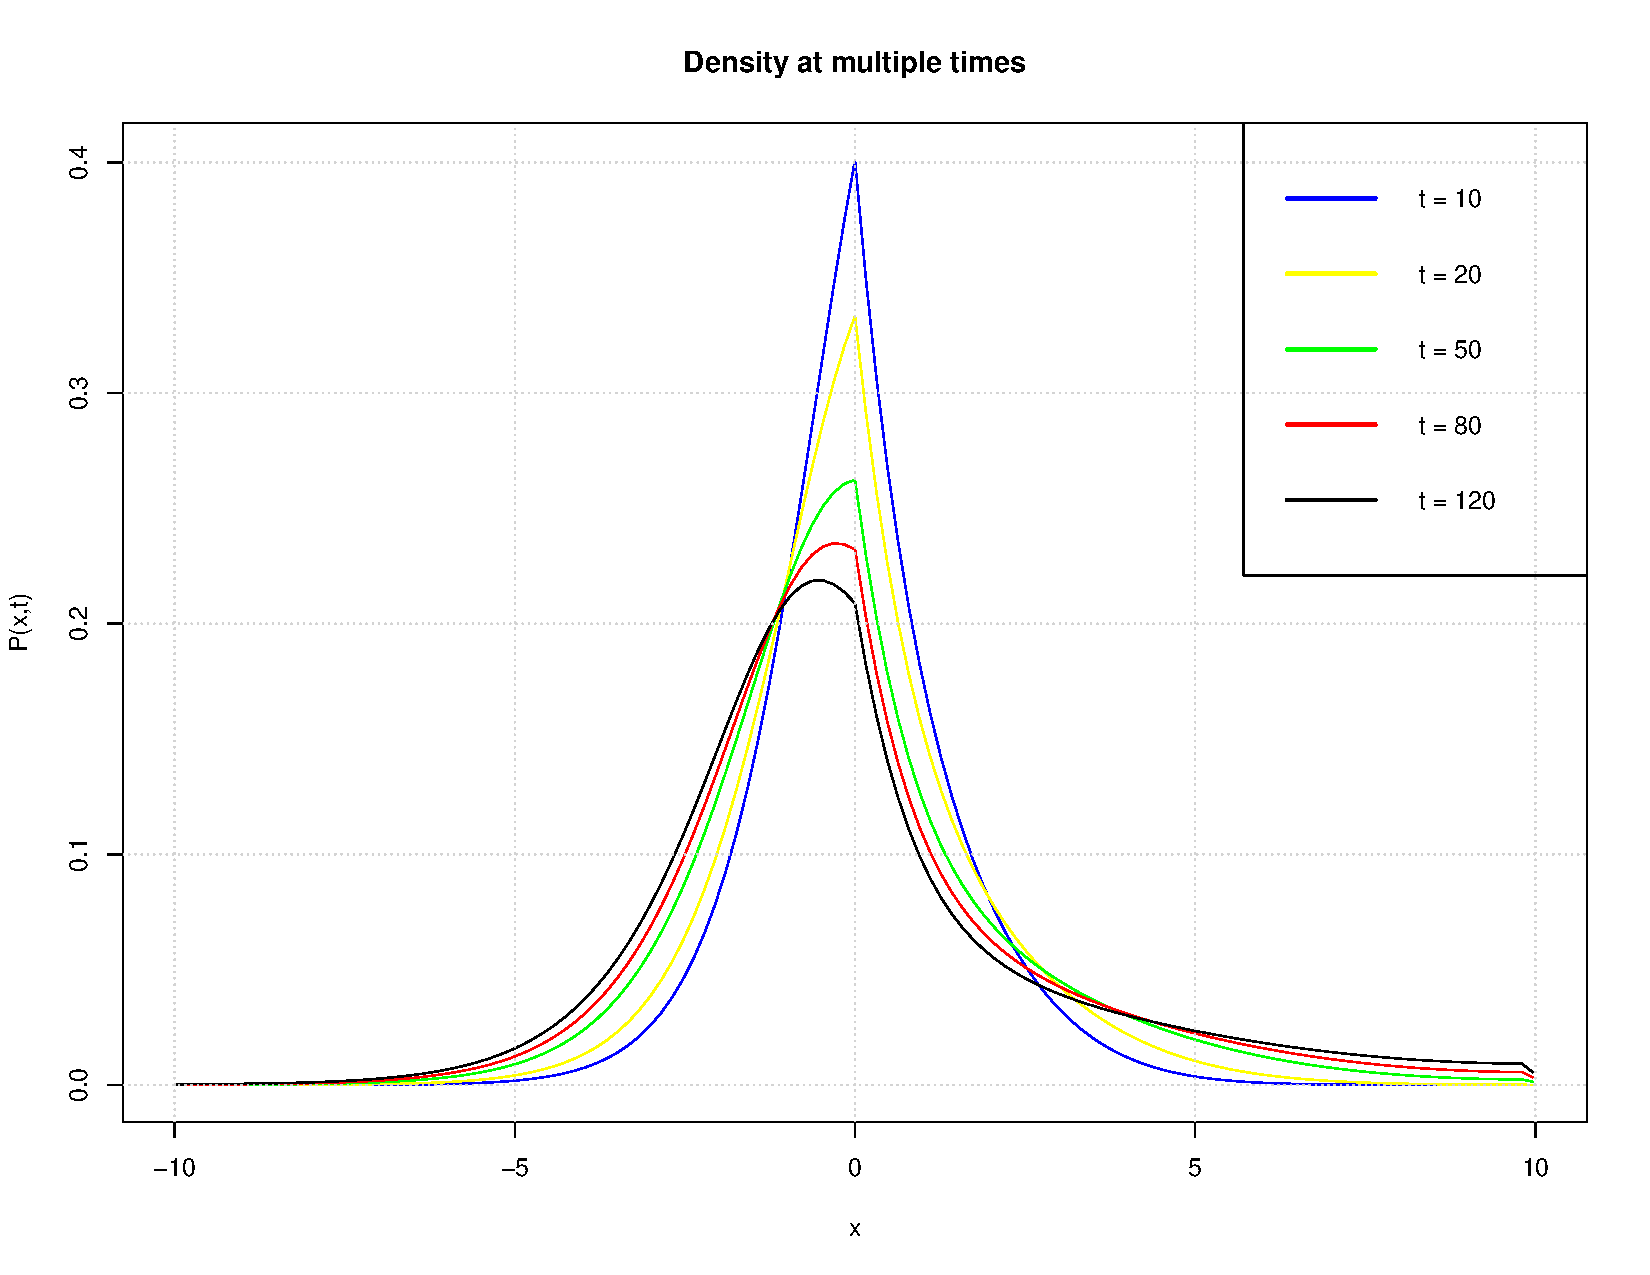
\includegraphics[scale=0.6]{varyexp1}
\caption{\label{fig:varyexp1}
Density $P(x,t)$ at multiple times of a variable order subdiffusive system with $\beta(x) = 0.25 + 0.5/(1+e^{-x})$. The time scale $T_0 = 2$ and $c = 40$.}
\end{figure}

\begin{figure}[h]
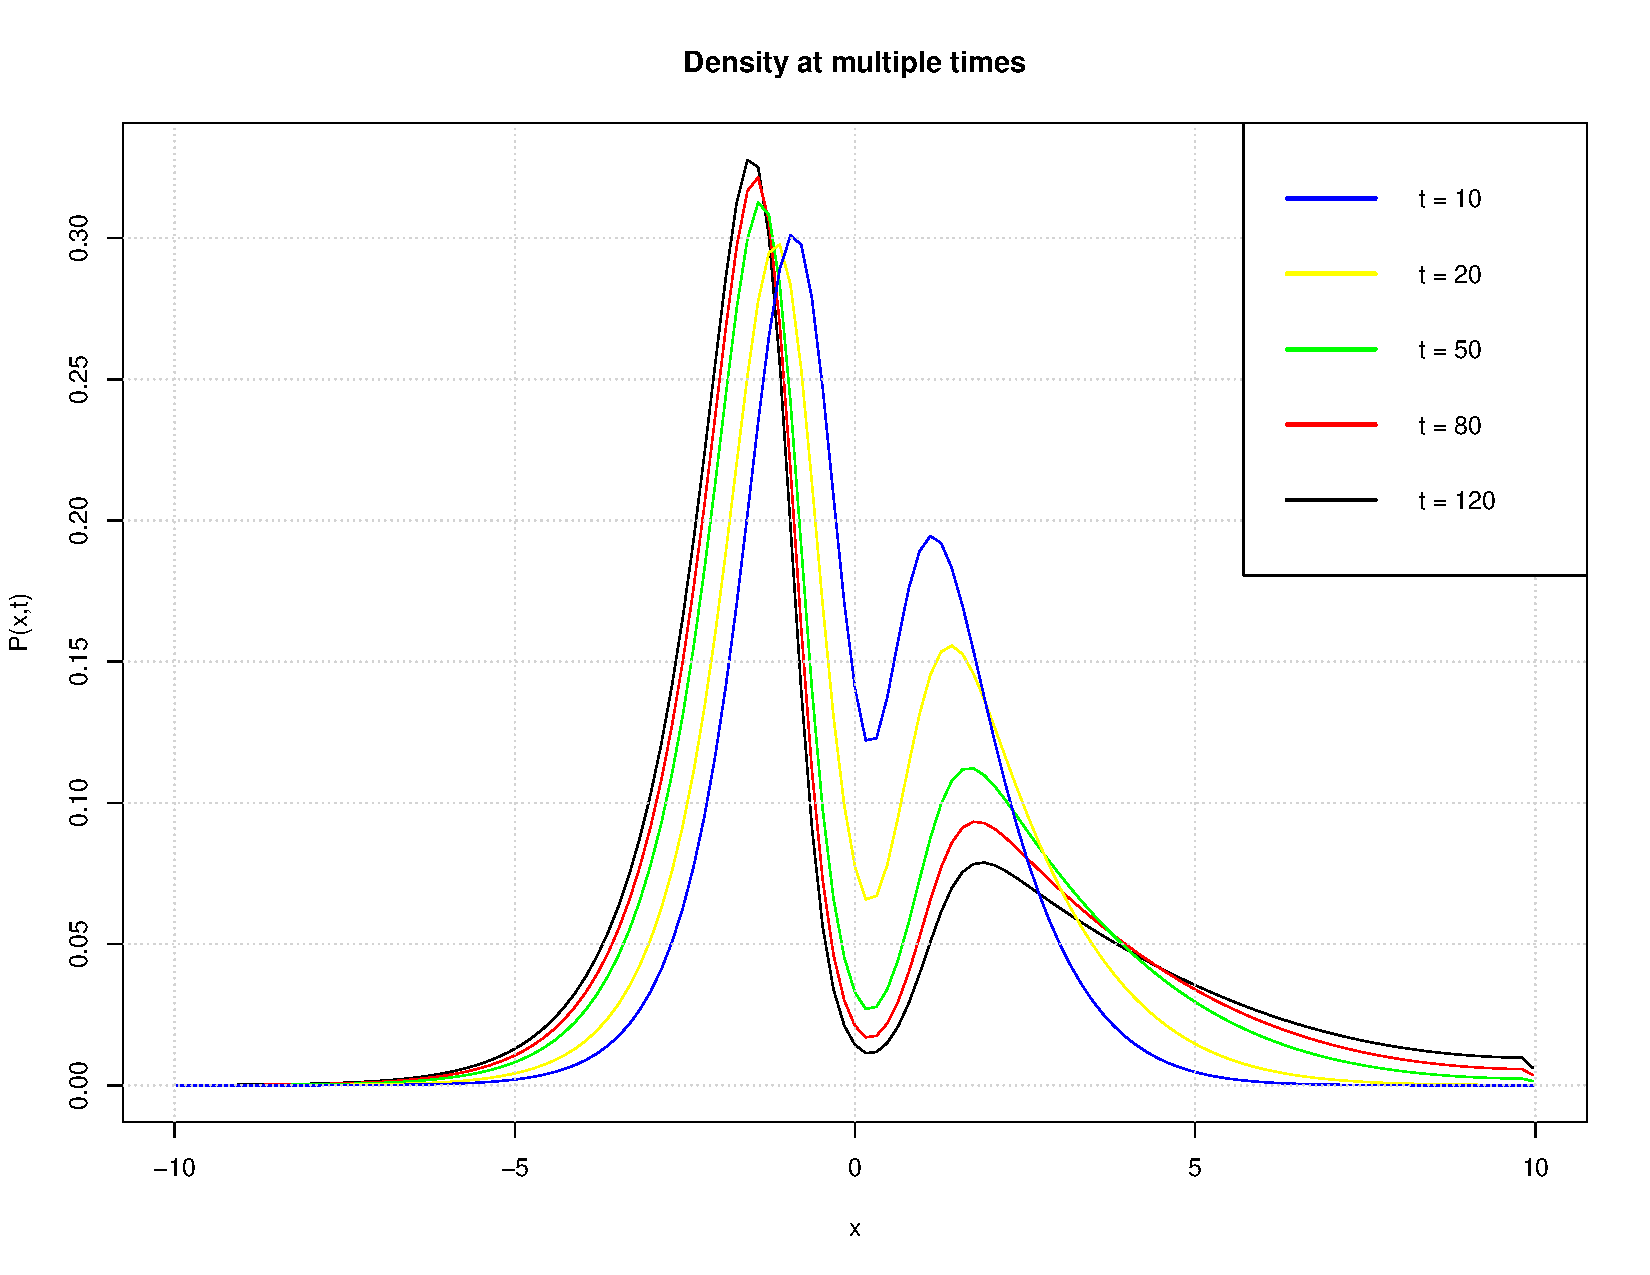
\includegraphics[scale=0.6]{varyexp2}
\caption{\label{fig:varyexp2}
Density $P(x,t)$ at multiple times of a variable order subdiffusive system with $\beta (x) = 0.55e^{-x^2} + 0.15 + 0.5/(1+e^{-2x})$. The time scale $T_0 = 2$ and $c = 40$.}
\end{figure}


\paragraph{Spatially varying Tempering}  The tempered Tail function is obtained by multiplying it by an exponential term $e^{-\theta  t}$. This yields the new Tail function $\Psi(x,t) = \frac{t^{-\beta(x)} e^{-\theta  t}}{\Gamma (1-\beta(x))}$ where $\theta \geq 0$ and we can see that this Tail function will now be integrable. Note that for $\theta = 0$ this reduces to the original tail function, and observe that for small $t$ and small $\theta$ dynamics of the system will still appear subdiffusive, while for large $t$ they will approach diffusive. Here we are now able to generalize this to allow the tempering parameter $\theta (x) \geq 0$ to be spatially varying so that the effect of this tempering may not be homogeneous throughout the system. Taking the variable order to be the same as in Figure \ref{fig:varyexp1} $\beta(x) = 0.25 + 0.5/(1+e^{-x})$, we consider the inhomogeneous tempering $\theta (x) = 1/(1+e^{0.5x})$. Figure \ref{fig:varytempering} illustrates the density $P(x,t)$ for this case, where we can see that particles begin to accumulate where tempering is low $(x>0)$. Noting that the variable exponent $\beta(x)$ is lower for $x<0$, this suggests that the effect of the tempering parameter $\theta (x)$ is stronger than that of $\beta(x)$. \\

\begin{figure}[h]
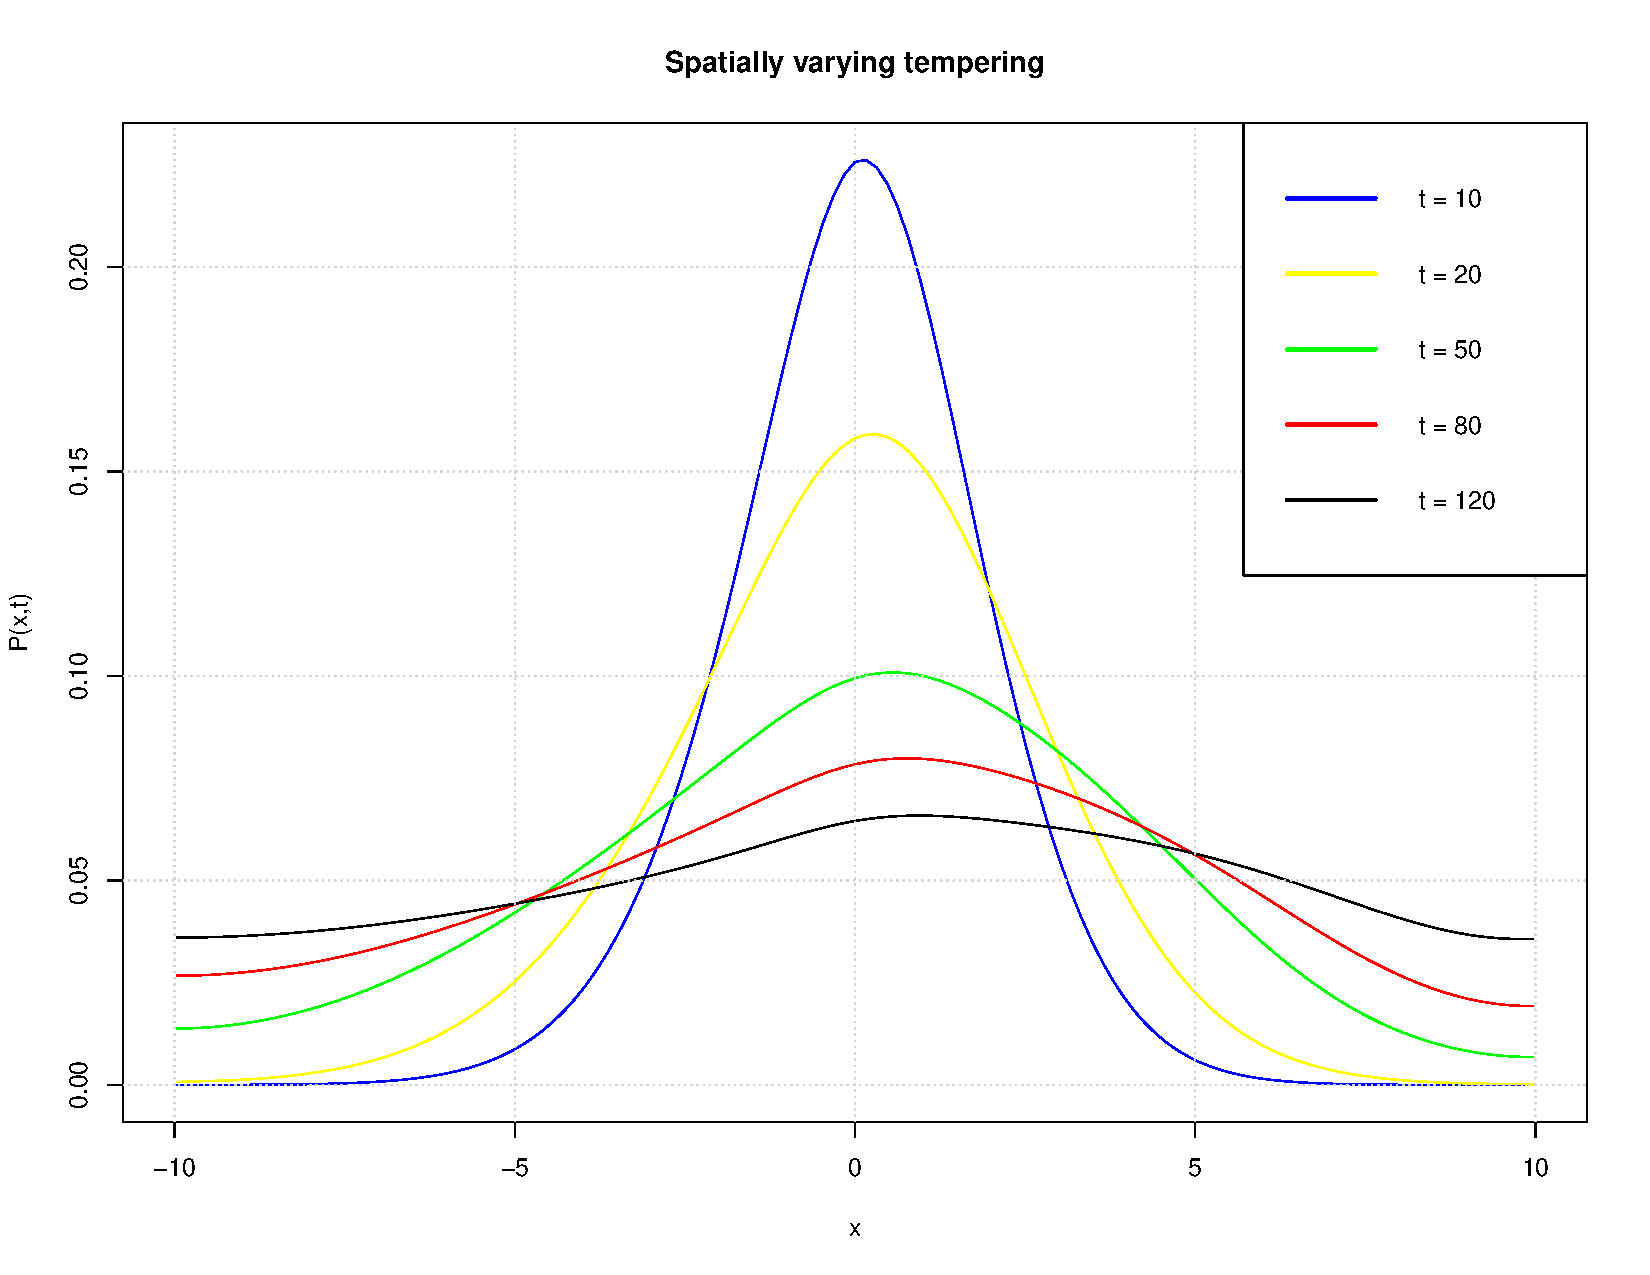
\includegraphics[scale=0.6]{varytempering}
\caption{\label{fig:varytempering}
Density $P(x,t)$ at multiple times of a variable order subdiffusive system with spatially varying tempering. We set $\beta(x) = 0.25 + 0.5/(1+e^{-x})$ and $\theta (x) = 1/(1+e^{0.5x})$. The time scale $T_0 = 2$ and $c = 40$.}
\end{figure}



\section{Conclusion}

\section*{References}

\bibliography{varyExp}



\end{document}
